\documentclass[12pt,titlepage,twoside]{article}
\usepackage{titlesec}

\usepackage{blindtext}

\usepackage{german}				% deutsche Überschriften etc.
\usepackage[utf8]{inputenc}		% direkte Einbgabe von Umlauten

% Layout-Einstellungen
\frenchspacing					% no extra space after periods
\usepackage{parskip}			% paragraph gaps instead of indentation
\usepackage{mathptmx}			% supposed to replace \usepackage{times}
\usepackage[scaled=0.9]{helvet}	% supposed to replace \usepackage{times}
\usepackage{courier}			% supposed to replace \usepackage{times}
\tolerance=9000					% avoid words across right border

% miscellaneous
\usepackage{graphicx}			% save svg with dia -> use inkscape to save as pdf
\usepackage{rotating}
\usepackage{wrapfig}
\usepackage{hhline}				% double lines in tables
\usepackage{amsfonts}			% real numbers etc.
\usepackage[rightcaption]{sidecap}	% figure captions on the right (optional)
\usepackage{listings}			% for code samples
\lstset{
    escapeinside={(*@}{@*)}
}
\renewcommand{\lstlistlistingname}{Listingverzeichnis}	% header name for the list of listings

\usepackage{fancyhdr}			% for header line
\usepackage{booktabs}
\usepackage{float}

\usepackage{diagbox}			% diagonal table cell lines

\usepackage{geometry}

\geometry{a4paper,left=25mm, right=25mm, top=3.0cm, bottom=2.5cm}
\usepackage{tabularx}
% Kopf- und Fußzeile
\fancyhead{} % clear all header fields
\fancyhead[OR,LE]{\leftmark}

\usepackage{hyperref}			% for clickable references
\hypersetup{
	linktoc=all,
	colorlinks,
	citecolor=black,
	filecolor=black,
	linkcolor=black,
	urlcolor=black,
	plainpages=false
}

\usepackage{cite}
\renewcommand{\UrlBreaks}{\do\/\do\-\do\_}	% allows URL breaking on /, - and _
\usepackage{breakurl}

\usepackage[toc,page]{appendix}
\usepackage[nottoc]{tocbibind}

\usepackage{etoolbox}	% may already be loaded by bibtex
\patchcmd{\thebibliography}{\clubpenalty4000}{\clubpenalty10000}{}{}	% avoid breaking bib entrys
\patchcmd{\thebibliography}{\widowpenalty4000}{\clubpenalty10000}{}{}	% avoid breaking bib entrys

\newlength\tdima
\newcommand\tabfill[1]{
      \setlength\tdima{\linewidth}
      \addtolength\tdima{\@totalleftmargin}
      \addtolength\tdima{-\dimen\@curtab}
      \parbox[t]{\tdima}{#1\ifhmode\strut\fi}}

\newcommand*{\reflabel}[1]{\hyperref[{#1}]{\ref*{#1} \nameref*{#1}}}
\newcommand*{\reftype}[1]{\hyperref[{#1}]{\autoref*{#1}}}
\newcommand*{\refcomplete}[1]{\hyperref[{#1}]{\autoref*{#1} \nameref*{#1}}}

\renewcommand{\contentsname}{Inhaltsverzeichnis}
\renewcommand\appendixtocname{Anhang}
\renewcommand\appendixpagename{Anhang}

\def\postbreak{
  \raisebox{0ex}[2.0ex][0.5ex]{\ensuremath{\color{red}\hookrightarrow\space}}}

\lstdefinelanguage{JavaScript}{
  keywords={typeof, new, true, false, catch, function, return, null, catch, switch, var, if, in, while, do, else, case, break},
  keywordstyle=\color{blue}\bfseries,
  ndkeywords={class, export, boolean, throw, implements, import, this},
  ndkeywordstyle=\color{darkgray}\bfseries,
  identifierstyle=\color{black},
  sensitive=false,
  comment=[l]{//},
  morecomment=[s]{/*}{*/},
  commentstyle=\color{purple}\ttfamily,
  stringstyle=\color{red}\ttfamily,
  morestring=[b]',
  morestring=[b]"
}

\title{Titel: Design und Implementierung einer Serverless Infrastructure Anwendung beim Cloud Anbieter Amazon Web Services}
\newcommand{\titleEnglish}{English title}

\author{Oktavius Wiesner}
\newcommand{\Matrikelnummer}{1082104}
\date{\today{}, Duisburg}

\makeatletter
%%%%%%%%%%%%%%%%%%%%%%%%%%%%%%%%%%%%%%%%%%%%%%%%%%%%%%%%%%%%
\begin{document}

\bibliographystyle{amsalpha}

\definecolor{dkgreen}{rgb}{0,0.6,0}
\definecolor{gray}{rgb}{0.5,0.5,0.5}
\definecolor{mauve}{rgb}{0.58,0,0.82}
\definecolor{lightgray}{rgb}{.9,.9,.9}
\definecolor{darkgray}{rgb}{.4,.4,.4}
\definecolor{purple}{rgb}{0.65, 0.12, 0.82}

\pagenumbering{roman}	% Start roman numbering - 'Roman' for uppercase


%-------------------------------------------------------------

\begin{titlepage}

\begin{center}
{\Large\bf \@title}\\[3cm]



{\bf Bachelorarbeit}\\
zur Erlangung des Grades {\em Bachelor of Science}\\[1.5cm]

an der\\
Hochschule Niederrhein\\
Fachbereich Elektrotechnik und Informatik\\
Studiengang {\em Informatik}\\[3cm]

vorgelegt von\\
\@author\\
Matrikelnummer: \Matrikelnummer\\[3cm]
Datum: \today\\[3cm]

Prüfer:~Prof.~Dr.~Peter Davids
\\Zweitprüfer:~Maik Glatki

\end{center}
\end{titlepage}

\pagestyle{empty}
\clearpage

%-------------------------------------------------------------


%-------------------------------------------------------------

%-------------------------------------------------------------
\section*{Zusammenfassung}
%-------------------------------------------------------------
Notwendig?

In dieser Bachelorarbeit werden folgende Themen behandelt:

- Cloud Computing und Servicemodelle

- Function as a Service

- Serverless Architektur

- Serverless Dienste beim Cloud Provider Amazon Web Services und Designentscheidungen

- Implementierung einer Webanwendung mit AWS Amplify und React

- Ausblick auf die Zukunft



%-------------------------------------------------------------
\section*{Abstract}
%-------------------------------------------------------------

Die vorliegende Bachelorarbeit beschäftigt sich im Detail mit Serverless Architektur und Function as a Service.
Zur Verständlichkeit werden die verschiedenen Servicemodelle des Cloud Computings vorgestestellt und verglichen.
Die Bachelorarbeit beschränkt sich auf den Cloud Provider Amazon Web Services und der entsprechenden Dienste, die für den Einsatz von Serverless Anwendungen zur Verfügung stehen.
Dabei werden AWS-Dienste wie Lambda, Cognito, AppSync, DynamoDB und Amplify genauer untersucht und bewertet.
Auf Basis der untersuchten Dienste wird ein Prototyp bei AWS entwickelt und implementiert. Die Programmiersprache ist bei der Implementierung NodeJS bzw. Javascript und React.
Das Ziel ist eine moderne Web Applikation für die Mitarbeiter der Mediengruppe RTL, die komplett auf Serverless Architektur basiert
und die in der Bachelorarbeit erwähnten Vorteile vollständig ausnutzen kann.




\clearpage

%-------------------------------------------------------------


%-------------------------------------------------------------

%-------------------------------------------------------------
\section*{Eidesstattliche Erklärung}
%-------------------------------------------------------------
%\begin{tabbing}
%Name: \hspace{4em}\= \@author\\
%Matrikelnr.: \> \Matrikelnummer\\
%Titel: \> \@title
%\end{tabbing}

\begin{table}[h]
\begin{tabularx}{\textwidth}{l X}
Name:			& \@author \\
Matrikelnr.:	& \Matrikelnummer \\
Titel:			& \@title

				\titleEnglish \\
\end{tabularx}
\end{table}

Ich versichere durch meine Unterschrift, dass die vorliegende Arbeit
ausschließlich von mir verfasst wurde.
Es wurden keine anderen als die von mir angegebenen Quellen und Hilfsmittel
benutzt.

Die Arbeit besteht aus \underline{\hspace{3em}} Seiten.

\vspace{8ex}
\begin{tabbing}
\underline{\hspace{14em}} \hspace{3em}\= \underline{\hspace{14em}} \\
Ort, Datum \> Unterschrift
\end{tabbing}





\clearpage





%-------------------------------------------------------------


%-------------------------------------------------------------
\section*{Hinweis}

Bei allen Ausführungen im Folgenden, die auf Personen bezogen sind, meint die
gewählte Formulierung beide Geschlechter, auch wenn aus Gründen der
sprachlichen Vereinfachung und der besseren Lesbarkeit die männliche Form
gewählt wurde.

\cleardoublepage
%-------------------------------------------------------------


%-------------------------------------------------------------
\section*{Danksagung}

Hier kommt eine Danksagung...






\clearpage
%-------------------------------------------------------------

\pagestyle{fancy}
\tableofcontents

\clearpage
\pagestyle{empty}

\clearpage


%-------------------------------------------------------------
% default a), b), c) numbering
\renewcommand{\labelenumi}{\alph{enumi})}
\pagenumbering{arabic} % Switch to regular numbers
%=============================================================


%%%%%%%%%%%%%%%%%%%%%%%%%%%%%%%%%%%%%%%%%%%%%%%%%%%%%%%%%%%%%%%%%%%%%%%%%%%%%%%%
\pagestyle{fancy}
\fancyhf{}

\fancyhead[OR]{Einleitung}
\fancyhead[ER]{Einleitung}


\section{Einleitung}

\subsection{Aufgabenstellung}

Das Ziel dieser Bachelorarbeit ist es die Serverless-Architektur zu bewerten und einen Prototyp für die Abteilung Datacenter and Clouds der Firma CBC Cologne Broadcasting Center GmbH (Im folgenden \glqq CBC\grqq) zu erstellen.
Der Fokus soll hierbei gleichmäßig auf das Design der Anwendung sowie der Implementierung gelegt werden.

Im ersten Schritt soll überprüft werden, inwieweit sich die gewünschte Anwendung mit Serverless-Diensten realisieren lässt.
Anschließend sollen alle potenziellen Dienste des Cloud Providers Amazon Web Services (Im folgenden \glqq AWS\grqq) untersucht werden und die geeignetsten ausgewählt werden.

Bei der Implementierung sollen diese Dienste dann in der Praxis angewandt werden. Für das Frontend soll ein modernes Framework verwendet werden.
Die Implementierung soll möglichst allgemein verwirklicht werden, sodass jeder Mitarbeiter der Abteilung Datacenter and Clouds in Zukunft an dieser Anwendung weiter arbeiten kann.

Im Rahmen der Bachelorarbeit sollen alle Grundfunktionen umgesetzt werden, sodass in Zukunft weitere Funktionalitäten leicht ergänzt werden können.
Der Prototyp muss über eine Authentifizierung verfügen und Informationen zu bestehenden AWS Accounts (siehe \textit{\ref{Accountstruktur} \nameref{Accountstruktur}}) anzeigen können.

Für ein besseres Verständnis wie genau der Prototyp aussehen soll, kann es helfen die Abbildung im Abschnitt \textit{\ref{FertigSeite} \nameref{FertigSeite}} bereits zu Beginn zu betrachten.



\subsection{Motivation}
\label{Motivation}
Die Abteilung Datacenter and Clouds innerhalb von CBC beschäftigt sich mittlerweile seit einigen Jahren mit Cloud Infrastruktur.
Zu Beginn wurden größtenteils dynamisch Linux Server mit einer Datenbank und einem Loadbalancer realisiert(Infrastructure as a Service).
Mit der Zeit wurden auch containerbasierte Varianten mit Docker sowie Platform as a Service Lösungen umgesetzt.
Function as a Service wurde bisher nur mit dem Dienst Lambda (siehe \textit{\ref{Lambda} \nameref{Lambda}}) von AWS realisiert.
Mittlerweile gibt es den Wunsch sich intensiv mit Function as a Service zu beschäftigen um vor allem eine schnelle Bereitstellung von Diensten mit geringen Kosten zu ermöglichen.
Webanwendungen sollen schneller bereitgestellt werden, ohne dass Server konfiguriert und gewartet werden müssen.
Eine genau Erläuterung der genannten \glqq [...] as a Service\grqq{} Begriffe befindet sich im Kapitel \textit{\ref{Servicemodelle} \nameref{Servicemodelle}}.

Da sehr viele Firmen innerhalb der Mediengruppe RTL intensiv mit AWS und anderen Cloud Providern arbeiten ist die Kostenzuweisung unübersichtlich geworden.
Jeder Cloud Provider stellt Informationen zu Kosten und Abrechnungen auf unterschiedliche Weise dar und alle Daten müssen unterschiedlich aufbereitet werden.
AWS z.B. exportiert die Abrechnungen fortlaufend in dem Cloud-Speicher
S3\footnote{S3 steht für Simple Storage Service und ist ein Objektspeicherservice für eine beliebe Menge von Daten.
Daten werden in S3 Buckets abgelegt und können aus dem Internet abgerufen werden.
CBC verwendet S3 für viele unterschiedliche Szenarien, darunter auch das Speichern von Videodateien für den Dienst TVNOW.   }, wohingegen Google Cloud Plattform alle Daten in einem zentralen Datenbanksystem speichert.
Es ist notwendig die Kosten den Mediengruppe RTL-Abteilungen zuzuweisen.

Deshalb besteht innerhalb der Abteilung Datacenter and Clouds der Wunsch nach einer modernen Web Applikation, welche die Informationen der jeweiligen Cloud Provider zentral sammelt und zur Verfügung stellt.
Zu den Informationen gehören Daten zu den Kosten, Abrechnungen, verwendete Ressourcen und nach Bedarf weitere.
Im Rahmen der Bachelorarbeit soll dafür ein Prototyp entstehen der effizient und einfach in Zukunft um weitere Anforderungen erweitert werden kann.


\subsection{CBC Cologne Broadcasting Center GmbH}

Die Bachelorarbeit wird innerhalb der Räumlichkeiten des Unternehmens CBC Cologne Broadcasting Center GmbH in Köln Deutz realisiert.
CBC ist ein Unternehmen der Mediengruppe RTL Deutschland, welches wiederum zur Bertelsmann-Tochter RTL Group in Luxemburg gehört.
Neben CBC gehören unter anderem der Werbezeitenvermarkter IP Deutschland sowie die Fernsehsender RTL Television, RTL Nitro, N-TV und Vox zur Mediengruppe RTL.


Mit ca. 550 festen Mitarbeitern ist CBC für die Produktion, Programmverbreitung, Sendeabwicklung sowie die IT Infrastruktur verantwortlich.
Neben der Betreuung von Projekten innerhalb der Mediengruppe RTL ist die CBC auch für Produktion und Broadcast der Berichterstattung der Fußball-Bundesliga verantwortlich.
Die Abteilung Datacenter and Clouds beschäftigt sich dabei mit Infrastrukturthemen, sowohl On Premises als auch bei den Cloud Providern Amazon Web Services, Microsoft Azure sowie Google Cloud Platform.
Beispiele für Projekte, die in der Cloud umgesetzt wurden sind die Streaming-Plattform TVNOW sowie die Internetpräsenz des Nachrichtensenders N-TV.
Gegründet wurde die CBC 1994 in Köln, Geschäftsführer ist Thomas Harscheidt.

\clearpage
\section{Theorie}

\subsection{Definition und Pradigmen}

Was genau ist Serverless?

Serverless bedeutet... blaa blaaa blaa...


%%%%%%%%%%%%%%%%%%%%%%%%%%%%%%%%%%%%%%%%%%%%%%%%%%%%%%%%%%%%%%%%%%%%%%%%%%%%%%%%


\clearpage
\fancyhead[OR]{Fazit}
\fancyhead[ER]{Fazit}
\fancyfoot[C]{\thepage} %Seitennummer

\section{Fazit}

\subsection{Diskussion}

Ziel dieser Bachelorarbeit war es, die Serverless Architektur zu betrachten, und nach einer umfangreichen Betrachtung aller Dienste, einen Prototyp beim Cloud Provider AWS zu entwickeln.
Ein wichtiges Merkmal war zudem, dass die Möglichkeit vorgesehen ist, dass die Webanwendung in Zukunft ohne viel Aufwand um weitere Funktionalitäten ergänzt werden kann.
Die Wartung und Administration der Infrastruktur sollte dabei nach Möglichkeit so weit wie möglich vom Cloud Provider übernommen werden.

Im Rahmen der Bachelorarbeit lag der Fokus insbesondere auf die Designentscheidungen der einzelnen Dienste sowie eine grundsätzliche Funktionalität der Anwendung.
Dazu gehören eine sichere Möglichkeit zur Authentifizierung sowie eine Backend-Logik, die bestimmte Daten abrufen und verarbeiten kann.
Es ist sichergestellt, dass nur zugelassene Mitarbeiter die Anwendung nutzen können.
Außerdem sollte das Web Frontend eine Übersicht über alle Daten darstellen können und bei Bedarf leicht angepasst werden.
Neben dem Aspekt sich hauptsächlich um die Programmierung der Webanwendung zu kümmern, und nicht die zugrundeliegende Infrastruktur, sollten auch unnötige Kosten vermieden werden.
Da die meisten Dienste nach benötigten Anforderungen abgerechnet werden, können die Kosten auf ein Minimum gehalten werden.
Diese Ziele wurden erreicht. Die genaue Übersicht der Kosten folgt im nächsten Abschnitt.

Eine Integration mit Unternehmensidentäten war zum Zeitpunkt leider nicht umsetzbar.
Zum einem würde der Aufwand den gesetzten Rahmen für die Bachelorarbeit deutlich überschreiten, zum anderem entspricht der potenzielle Lösungsvorschlag nicht den Wünschen.

Die gründliche Auseinandersetzung mit den einzelnen Diensten stellte sich als äußerst nützlich dar.
Durch die Abstraktion von Amplify ist nicht jeder Prozess im Detail ersichtlich und es kann schwerfallen den genauen Zusammenhang zu verstehen.
Dank der intensiven Prüfung im dritten Kapitel ist es leichter die Methodik der einzelnen Technologien zu begreifen.
Zugleich ermöglichst es die Verwendung der Dienste ohne Amplify, da genügend Verständnis geschaffen wurde.
Das erlangte Wissen über die Serverless Architektur kann als Vorlage für weitere Projekte genutzt werden.

Der Einsatz von Amplify ermöglichte eine bequemere und übersichtlichere Realisierung.
Viele Vorgänge wurden merklich beschleunigt.
Zudem war es so möglich innerhalb von kurzer Zeit eine vollständige serverlose Webanwendung mit den essentiellsten Funktionen zu entwickeln, die keine Wartung oder Administration benötigt.
\clearpage

\subsection{Kosten}
\label{Kosten}
Neben dem minimalen Aufwand zählen die Kosten ebenfalls zu den Vorteilen der Serverless Architektur.
Während des gesamten dritten Kapitels wurden Informationen zur Abrechnung der einzelnen Dienste aufgestellt.
Viele Dienste bieten kostenlose Kontingente an.
Dies führt vor allem zu extrem geringen Kosten während der Entwicklungsphase.

Das folgende Bild bestätigt diese Annahme.
In den Monaten August und September sind nur Kosten für die Dienste AppSync und DynamoDB entstanden.
Lambda, Amplify und Cognito sind während des Zeitraums ohne Kosten genutzt worden.
Die Kosten für September belaufen sich auf 0.12 USD für AppSync und 0.02 USD für DynamoDB.
Im August sind die Kosten vergleichbar.
Sobald die Anwendung produktiv genutzt wird, und die kostenlosen Kontingente aufgebraucht sind, steigen die Kosten.

Zur Zeit kann der Eindruck bestätigt werden, dass die Kosten mit Serverless Diensten gering gehalten werden können.
Eine vergleichbare Anwendung für ca. 0.15 USD pro Monat ist ohne den Einsatz der Serverless Architektur nur sehr schwer bis gar nicht realisierbar.
Wie sich die Kosten bei intensiver Nutzung verhalten muss zu einem späteren Zeitpunkt erneut evaluiert werden.
Eine exakte Prognose ist schwierig.
Bis auf einen Anstieg der Kosten bei AppSync reichen vermutlich die meisten kostenlosen Kontingente auch während der Anfangszeit aus.
Das Kontingent von Cognito mit 50.000 Nutzern wird mit großer Wahrscheinlichkeit nie aufgebraucht.
Sobald eine Anmeldung mit Unternehmens-Identitätsanbieter möglich ist, kann die Anzahl der Nutzer jedoch schnell über das deutliche kleinere Kontingent von 50 Nutzern überschritten werden.
Auch bei Lambda und DynamoDB wird, sofern keine weitere Funktionalität implementiert wird, kein großer Anstieg erwartet.
Geht man von eine Millionen API-Aufrufen pro Monat aus, würden die Kosten für AppSync bei 4,00 USD liegen.
\\
\begin{figure}[htbp]
    \centering
    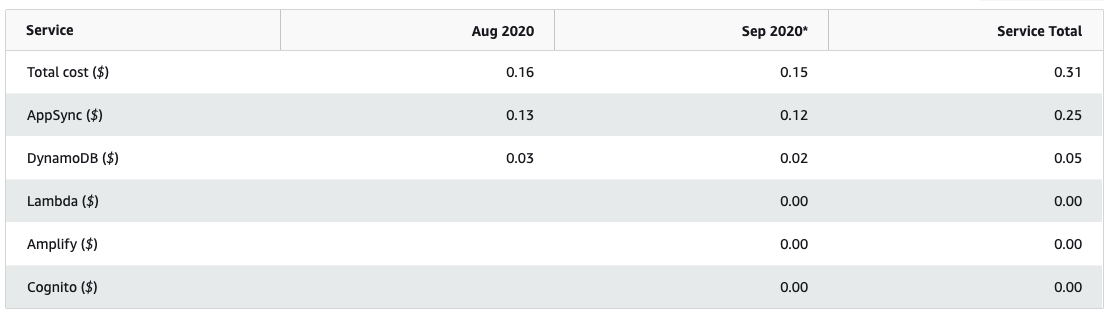
\includegraphics[width=1.0\textwidth]{50-Implementierung/Kosten.png}
    \caption{Kostenaufstellung der letzten zwei Monate}
    \label{fig:kosten}
\end{figure}
\clearpage

\subsection{Zusammenfassung}
Im Rahmen dieser Bachelorarbeit wurde die Serverless Architektur analysiert und ein funktionsfähiger Prototyp entwickelt.
Als Motivation gilt ein steigendes Interesse an Function as a Service Diensten sowie an einer schnelleren Bereitstellung von Diensten.
Die Kostenübersicht aller Cloud-Provider der Mediengruppe RTL soll vereinfacht werden und zentral aufbereitet werden.
Damit geht die Anforderung einher eine einfache und administrationsfreie Realisierung zu ermöglichen, die im besten Fall keine hohen Kosten verursacht.
Um eine qualifizierte Aussage zu einer Implementierung mit Serverless Diensten geben zu können, wurden im Voraus die wichtigsten Cloud Computing-Modelle erläutert und den Zusammenhang zu Serverless erklärt.
Im Anschluss wurde die Serverless Architektur auf ihre Eignung geprüft und bestätigt.
Die Umsetzung sollte möglichst von nur einer Person erfolgen, ohne Expertenwissen in jedem Fachgebiet zu erfordern.

Da es mehrere mögliche Ansätze zur Umsetzung gibt, ist es besonders wichtig die einzelnen Möglichkeiten zu vergleichen.
Aus diesem Grund wurden im Rahmen der Bachelorarbeit einzelne Dienste des Cloud Providers AWS untersucht und miteinander verglichen.
Nachdem die zugrundeliegende Technologie des Dienstes und der Funktionsumfang des Dienstes geprüft wurden, konnte schließlich eine Entscheidung gefällt werden.
Die einzelnen zu prüfenden Bereiche beschäftigten sich mit den Themen API, Datenbanken, Backend-Logik und Authentifizierung.
In jedem Bereich wurde ein passender Dienst ausgewählt und im weiteren Verlauf auch implementiert.
Als API wurde der AWS Dienst AppSync genutzt, der auf GraphQL basiert.
Der Dienst AWS Cognito übernimmt die Authentifizierung und Absicherung der Anwendung.
Als relationale Datenbank kommt der Dienst AWS DynamoDB zum Einsatz.
Die Backend-Logik wird mit dem Function as a Service Dienst AWS-Lambda realisiert.
Das Frontend wurde mit dem JavaScript-Framework React erstellt.
AWS Amplify dient als zentraler Dienst, um alle zuvor genannten Komponenten an zentraler Stelle konfigurieren zu können.

Das Ziel des Prototyps war es, eine funktionale Webanwendung zu erzeugen die eine Übersicht über alle aktiven AWS Accounts liefert.
Dafür musste ein Accountübergreifender Zugriff eingerichtet werden, da sich die benötigten Daten in einem anderen Account befinden als die Anwendung selbst.
Die gesammelten Daten speichert die Lambda-Funktion in eine DynamoDB-Tabelle ab.
Auf diese Daten greift das Frontend über die API zu, und erstellt mithilfe von React eine übersichtliche Tabelle aller Daten.
Da die gesamte Webanwendung im Internet erreichbar ist, wurde mit AWS Cognito eine Authentifizierung sichergestellt.
Registrierte Nutzer können die Webanwendung nutzen und auf die Daten zugreifen.

Während der Entwicklung wurde darauf geachtet eine möglichst einheitliche Programmiersprache zu verwenden.
Aufgrunddessen können andere Kollegen der Abteilung Datacenter and Clouds, ohne viel Einarbeitung, an dieser Webanwendung weiterentwickeln.
Zudem ist dank Anbindung an den Dienst GitHub eine gemeinsame Bearbeitung mühelos möglich.
Die Versionsverwaltung ermöglicht es zudem leicht Änderungen nachzuvollziehen.









\newpage
\subsection{Ausblick}
Das gesammelte Wissen über die Serverless Architektur sowie über alle gewählten Dienste kann in Zukunft ebenfalls bei weiteren Projekten von Datacenter and Clouds angewandt werden können.
Für künftige Projekte kann nun entschieden werden, ob sich eine Umsetzung mit Serverless Diensten anbietet oder ob die Realisierung mit einem anderen Service-Modell besser geeignet ist.

Für die Webanwendung selbst wurde das Grundgerüst geschaffen und es kann in Zukunft von jedem Mitarbeiter der Abteilung Datacenter and Clouds erweitert werden.
Insgesamt gibt es mehrere Bereiche, in denen die Webanwendung ausgebaut werden kann.

Für den Cloud Anbieter AWS stehen API und grundlegenden Funktionalitäten bereits zur Verfügung.
Allen interessierten Mitarbeiter kann Zugriff zur Anwendung gewährt werden.
Da die Kosten der einzelnen AWS Accounts für die einzelnen Abteilungen interessant sind, könnte die Lambda-Funktion um diese Aufgabe erweitert werden.

Jeder AWS Account zeigt eine detaillierte Übersicht der Kosten im AWS CostExplorer an.
CostExplorer ist ein Dienst, der es ermöglicht detaillierte Berichte zu allen AWS-Kosten zu erstellen und analysieren.
Die Abbildung \textit{\ref{fig:kosten} \nameref{fig:kosten}} ist beispielsweise über die Webansicht des Dienstes generiert worden.
Mithilfe des CostExplorer SDKs können beispielsweise die Gesamtkosten der letzten Monate in einer Lambda-Funktion abgerufen werden.
Zur Realisierung wäre es notwendig in jedem einzelnen AWS Account eine IAM-Rolle mit einer Vertrauensstellung zur Lambda-Funktion zu erstellen.
Die Lambda-Funktion müsste anschließend die IAM-Rolle in jedem Account annehmen und die Abfragen gegen den CostExplorer Dienst ausführen.
Zusätzlich müssten sowohl Datenbank als auch das Frontend angepasst werden.
Diese Informationen könnten für die jeweiligen Kostenstellen interessant sein.

Weiterhin sollte in Zukunft erneut die Anmeldung über Unternehmensidentitäten in Betracht gezogen werden, falls es eine vorteilhaftere Methode zur Realisierung gibt.

Da bisher noch keine nützliche Auswertung von Log-Dateien oder Metriken existiert, sollte dies im weiteren Verlauf implementiert werden.

Neben AWS können auch andere Cloud Provider in die Anwendung integriert werden.
Mit einer weiteren Lambda-Funktion könnte auf Daten innerhalb der Google Cloud Platform oder Azure Cloud zugegriffen werden.
So wäre eine zentralisierte Stelle für alle Cloud Provider möglich.


















%%%%%%%%%%%%%%%%%%%%%%%%%%%%%%%%%%%%%%%%%%%%%%%%%%%%%%%%%%%%%%

%\addtocontents{toc}{\protect\newpage}	% new ToC page

\newpage
\interlinepenalty=10000	% try to avoid page-breaking entries
\fancyhead[OR]{Literatur}
\fancyhead[ER]{Literatur}

\bibliography{cite}


%%%%%%%%%%%%%%%%%%%%%%%%%%%%%%%%%%%%%%%%%%%%%%%%%%%%%%%%%%%%%%
\newpage
\fancyhead[OR]{Anhang}
\fancyhead[ER]{Anhang}


\clearpage
\setcounter{page}{0}

\renewcommand{\thepage}{A-\arabic{page}}

\begin{appendices}

\section{Anhang Teil 1}

\lstset{frame=tb,
	escapeinside={@}{@},
	language=Java,
	aboveskip=3mm,
	belowskip=3mm,
	showstringspaces=false,
	columns=flexible,
	basicstyle={\small\ttfamily},
	numbers=none,
	numberstyle=\tiny\color{gray},
	keywordstyle=\color{mauve},
	commentstyle=\color{dkgreen},
	stringstyle=\color{blue},
	breaklines=true,
	breakatwhitespace=true,
	tabsize=3,
	postbreak=\raisebox{0ex}[0ex][0ex]{\ensuremath{\color{red}\hookrightarrow\space}}
}

\begin{lstlisting}[caption={Formularmanipulation},
label=lst:Beispielcode 1] Formularmanipulation {

$( document ).ready(function() {


    if ( $('#TimeUnits').length )
    {
        $('#TimeUnits').autocomplete({ disabled: true });
    }


    var ITPROLABCurrentAction = $.getUrlVar('Action');

    if ( ITPROLABCurrentAction == 'CustomerTicketMessage' )
    {
        var ITPROLABQueue         = $( "#Dest option:selected" ).text();
        alert( ITPROLABQueue );

        if (ITPROLABQueue != 'ITPROLAB' ) {
            $('#ITPROLABServiceID').fadeOut();
        }
    }



$("<style>")
    .prop("type", "text/css")
    .html("\                                                                                                    
    [title=\"10-blue\"] {\                                                                                      
        background-color: blue;\                                                                                
        color: blue;\                                                                                           
        font-size: 1px;\                                                                                        
        opacity: 0.7;\                                                                                          
    }")
    .appendTo("head");
    
\end{lstlisting}

\section{Anhang Teil 2}

\lstset{frame=tb,
	escapeinside={@}{@},
	language=Perl,
	aboveskip=3mm,
	belowskip=3mm,
	showstringspaces=false,
	columns=flexible,
	basicstyle={\small\ttfamily},
	numbers=none,
	numberstyle=\tiny\color{gray},
	keywordstyle=\color{blue},
	commentstyle=\color{dkgreen},
	stringstyle=\color{mauve},
	breaklines=true,
	breakatwhitespace=true,
	tabsize=3,
	otherkeywords={BIGINT,TEXT},
	postbreak=\raisebox{0ex}[0ex][0ex]{\ensuremath{\color{red}\hookrightarrow\space}}
}

\begin{lstlisting}[caption={Formularmanipulation},
label=lst:Beispielcode 2 Perl] Report Skript {

#!/usr/bin/perl                                                                                                                                                                          
##                                                                                                                                                                                       
#  generate PDF from Latex Template LK.tex --> lk.tex --> lk.pdf                                                                                                                         
#  wird von machform formular aufgerufen.                                                                                                                                                
##                                                                                                                                                                                       

use CGI qw/:standard/;
use DBI;

my $debug = 0;



my $template;
my $german  = "LK/LK-D.tex";
my $english = "LK/LK-E.tex";
my $arabic  = "LK/LK-A.tex";
my $lk      = "LK/lk.tex";



my $message = "<pre>\n";
my $dbm = DBI->connect ( "dbi:mysql:$database:$server",$userid,$passwd ) || die "Could not connect to $database";


$stm = $dbm->prepare ( qq{ select id,element_1, element_2, element_5, element_6, element_7, element_8, element_10_1,element_12 from $table  ORDER by id DESC LIMIT 1 });
$stm->execute;
$stm->bind_columns(\$id,\$e1,\$e2,\$e5,\$e6,\$e7,\$e8,\$e10,\$e12);
if ($stm->fetch) {

    if ($e5 =~ /-/) {
        $e5 = substr ($e5,8,2) . "." . substr ($e5,5,2) . "." . substr ($e5,0,4);
    }
    $message .= " ID     = $e1\n";
    $message .= " Name   = $e2\n";
    $message .= " Datum  = $e5\n";
    $message .= " Adresse= $e6\n";
    $message .= " E      = $e7\n";
    $message .= " K      = $e8\n";
    $message .= " data   = $e10\n";
    $message .= " lang   = $e12\n";

}
else {
    $message .= " nicht gefunden\n";
}

printf "$message\n" if ($debug);

undef $stm;
undef $dbm;

    
\end{lstlisting}


\section{Anhang Lambda}

\lstset{frame=tb,
	escapeinside={@}{@},
	language=JavaScript,
	keywords={break, case, catch, continue, debugger, default, delete, do, else, false, finally, for, function, if, in, instanceof, new, null, return, switch, this, throw, true, try, typeof, var, void, while, with}, morecomment=[l]{//},
	morecomment=[s]{/*}{*/},
	morestring=[b]',
	morestring=[b]",
	ndkeywords={class, export, boolean, throw, implements, import, this},
	aboveskip=3mm,
	belowskip=3mm,
	showstringspaces=false,
	columns=flexible,
	basicstyle={\small\ttfamily},
	numbers=none,
	numberstyle=\tiny\color{gray},
	keywordstyle=\color{mauve},
	commentstyle=\color{dkgreen},
	stringstyle=\color{blue},
	breaklines=true,
	breakatwhitespace=true,
	tabsize=3,
	postbreak=\raisebox{0ex}[0ex][0ex]{\ensuremath{\color{red}\hookrightarrow\space}},
	keywordstyle=\color{blue}\bfseries,
	ndkeywordstyle=\color{darkgray}\bfseries,
	identifierstyle=\color{black},
	commentstyle=\color{purple}\ttfamily,
	stringstyle=\color{red}\ttfamily
}

\begin{lstlisting}[caption={Lambda-Code in NodeJS},
label=lst:LambdaCode,basicstyle=\ttfamily\small ] Lambda-Code {

  /* Amplify Params - DO NOT EDIT
	ENV
	REGION
Amplify Params - DO NOT EDIT */

var AWS = require('aws-sdk')
AWS.config.update({region: 'eu-central-1'});

var docClient = new AWS.DynamoDB.DocumentClient

// Create AWS Service Objects for Lambda User
const s3 = new AWS.S3({apiVersion: '2006-03-01'});
const sts = new AWS.STS();


// Create Hash of String for Primary Key
const crypto = require('crypto')


// DynamoDB Helper Function. Currently not used.
async function getAllDynamoDBItems(){
  let params = {
    TableName: 'Comments-ifdtxan4k5fglip5ynnopk6bky-dev',
   };

       console.log("Starting Function")
  try {
     var result = await docClient.scan(params).promise()
     console.log(JSON.stringify(result))
     console.log("Success")
  } catch (error) {
     console.log("FAILED")
     console.error(error);
  }
}

// DynamoDB Function to write all collected Data
 const writeAllDynamoDBItems = async (id,num,accountid,name,email,status) => {
  let params = {
    TableName: 'Account-ifdtxan4k5fglip5ynnopk6bky-dev',
    Item:{
      "id":id,
      "num":num,
      "accountid": accountid,
      "name": name,
      "email": email,
      "status": status
  }
   };

     console.log("Writing Account " + name)
  try {
    var result = await docClient.put(params).promise()
    console.log("Success")
  } catch (error) {
    console.log("Failed Writing Files:")
    console.error(error);
  }
}

// STS Function --> Get Current Identity
const getCallerIdentity =  (sts_identity) => {
  return  sts_identity.getCallerIdentity().promise();

};

// STS Function --> Assume Role from another AWS Account
const getCrossAccountCredentials = () => {
  return new Promise((resolve, reject) => {
    const timestamp = (new Date()).getTime();
    const params = {
      RoleArn: 'arn:aws:iam::298094174079:role/amplify-kumo-access-role',
      RoleSessionName: `New-Session-${timestamp}`
    };
    sts.assumeRole(params, (err, data) => {
      if (err) reject(err);
      else {
        resolve({
          accessKeyId: data.Credentials.AccessKeyId,
          secretAccessKey: data.Credentials.SecretAccessKey,
          sessionToken: data.Credentials.SessionToken,
        });
      }
    });
  });
}
// j helps to count all accounts
var j = 0;
var all_accounts = []

// Organizations Function --> List all Accounts
var data_all;
const listAllAccounts =  (identity,params) => {
  return new Promise((resolve, reject) => {

    identity.listAccounts(params, (err, data) => {
      const params = {
        //NextToken: 'abc'
     };
     if (err) reject(err); // an error occurred
      else {
        console.log("Saved all Accounts");

            for (var i=0, max=data.Accounts.length; i < max; i++) {
                //console.log("Count: " + j + " ID:" + data.Accounts[i].Id +" is: " +  data.Accounts[i].Name)
                j += 1;
                //all_accounts.push(data.Accounts[i].Name);
                let str1 = data.Accounts[i].Name;
                let str2 = data.Accounts[i].Id;
                let str3 = str1.concat(str2)

                let hash = crypto.createHash('md5').update(str3).digest("hex")

                all_accounts.push({id:hash, num:j, accountid:data.Accounts[i].Id, name:data.Accounts[i].Name ,email:data.Accounts[i].Email ,status:data.Accounts[i].Status});
        }

           if (data.NextToken != undefined) {
               console.log("There is more")

            params.NextToken = data.NextToken;
            // Both Resolve are needed here so that function can terminate successfull
            resolve( listAllAccounts(identity,params) )
        }
        else {
          console.log("ENDE ERREICHRT")
          //console.log(all_accounts)
          resolve (all_accounts);
      }

   }    // successful response
})
});
} ;

exports.handler = async (event) => {
try {
  // Get getCrossAccountCredentials and Call Service Objects from AWS
  var accessparams = await getCrossAccountCredentials();
  const cbc_master_sts =  new AWS.STS({
    credentials: accessparams
  });

  const cbc_master_orgs = new AWS.Organizations({
    credentials: accessparams,
    region: 'us-east-1'
  });

  //Check own and assumed Identity

  const msg_caller = await getCallerIdentity(sts)
  console.log("Username Current Identity: " + msg_caller.Arn)
  const msg_caller_org = await getCallerIdentity(cbc_master_sts)
  console.log("Username Assumed Identity: " + msg_caller_org.Arn)

  const all_acc = await listAllAccounts(cbc_master_orgs)
  const start = async () => {
    for (let element of all_acc) {
      await writeAllDynamoDBItems(element.id,element.num,element.accountid,element.name,element.email,element.status) ;
      //console.log(element);
    }
    console.log('Done');
  }

  await start();

}
catch(err){
  console.log("Error while Assuming Role from another Account. Message:  " + err)
}

    const response = {
        statusCode: 200,
        body: JSON.stringify('Hello from Lambda!'),
    };
    return response
};

\end{lstlisting}


\end{appendices}


%%%%%%%%%%%%%%%%%%%%%%%%%%%%%%%%%%%%%%%%%%%%%%%%%%%%%%%%%%%%%%%%%%%%%%%%%%%%%%%%


\end{document}
%%%%%%%%%%%%%%%%%%%%%%%%%%%%%%%%%%%%%%%%%%%%%%%%%%%%%%%%%%%%%%%%%%%%%%%%%%%%%%%%
%%%%%%%%%%%%%%%%%%%%%%%%%%%%%%%%%%%%%%%%%%%%%%%%%%%%%%%%%%%%%%%%%%%%%%%%%%%%%%%%
%%%%%%%%%%%%%%%%%%%%%%%%%%%%%%%%%%%%%%%%%%%%%%%%%%%%%%%%%%%%%%%%%%%%%%%%%%%%%%%%
\makeatother
